

\begin{enumerate}
\item To what extent do workers within the same occupational category and with comparable skill sets engage in similar versus differentiated tasks, and how does this vary by gender?
\item Do wage differentials exist among workers performing the same tasks, and how are these differences moderated by both occupational context and gender?
\item What are the observable patterns of occupational and task segregation along gender lines, and how do these patterns contribute to the overall wage gap?
\end{enumerate}


\textcite{goldinGrandGenderConvergence2014a} highlights the need to look within occupations
to understand how jobs are organized and compensated and how this might diferentially affect men and
women. 

Within-occupational gender differences might also
persist, even after conditioning on differences in human capital and occupational choices. \textcite{cortes2018occupation}

A commonly used measure to summarize differences in the distribution of women and men across occupation categories 
is the index of segregation developed by Duncan (1955). 



The index of occupational segregation by sex is computed as

\begin{equation}
    D = 0.5 \sum_j |M_j - F_j|,
\end{equation}

where $M_j$ ($F_j$) is the fraction of all employed males (females) who work in occupation $j$. 
The index, which ranges between zero and one, indicates the proportion of women or men that would need 
to change occupations for the occupational distribution of men and women to be the same. In other words, 
if the distribution of men and women across occupational categories were identical (complete integration), 
the segregation index would equal zero. If all the occupations were either completely male or completely female 
(complete segregation), the segregation index would equal one.

\begin{figure}[!t]
    \centering
    \caption{Title}
    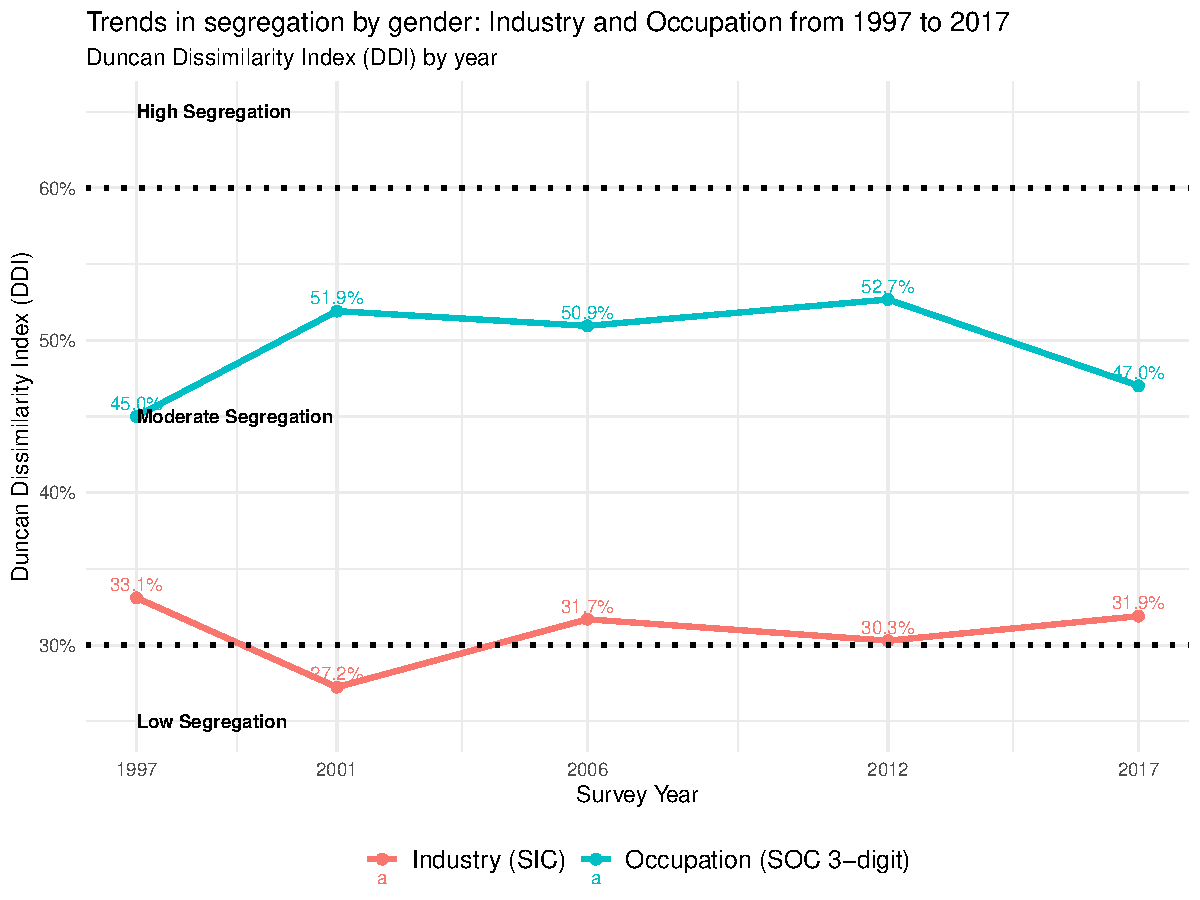
\includegraphics[width=\textwidth]{_graphic/industry_occupation3d_segreggation_fulltime.pdf}
    \label{fig:industry_occupation3d_segreggation_fulltime}
    \vspace{-3em}
    \justify\singlespacing\scriptsize\textit{Notes}: Notes here.
\end{figure}


The evolution of gender segregation in the UK labor market from 1997 to 2017 reveals persistent disparities
 in the distribution of men and women across both occupations and industries. Using the Duncan Dissimilarity 
 Index (D-index), I find that occupational segregation—measured at the 3-digit SOC level—remains consistently 
 moderate to high, with values ranging from 45.0\% in 1997 to 52.7\% in 2012, before declining slightly to 47.0\% 
 in 2017. These figures suggest that nearly half of either male or female workers would need to change occupations 
 to achieve gender parity, highlighting substantial and enduring occupational sorting by gender.

By contrast, industrial segregation—based on 2-digit SIC codes—remains lower and more stable, fluctuating 
between 27.2\% and 33.1\% over the same period. While both forms of segregation exhibit some variation, 
there is no strong or consistent trend toward greater integration over the 20-year span.

These results align with recent research documenting the persistence of occupational segregation despite 
broader gains in gender equality in education and employment. Studies such as England (2010), Blau and Kahn (2017), 
and Oesch et al. (2020) emphasize that, even as gender gaps in labor force participation and earnings have narrowed, 
occupational sorting continues to play a central role in maintaining inequality. Similarly, ILO (2021) and 
Rubery and Tavora (2020) note that gendered occupational patterns remain entrenched, even within high-skilled sectors. 
UK-specific analyses based on SES data (e.g., Green and Henseke, 2021) reinforce the view that occupational clustering 
and gendered task content have proven resilient. The higher and more variable levels of segregation observed at the 
occupational level underscore the value of disaggregated classifications such as 3-digit SOC codes in capturing 
structural barriers to gender integration.


\begin{table}[!t]
    \centering
    \caption{Task measures from the Skills and Employment Survey}
    \label{tab:task-ses}
    % \resizebox*{\textwidth}{!}{
    \begin{threeparttable}
        % \setlength{\tabcolsep}{6pt}
        % \small
        \begin{tabular}{@{}p{4cm}p{11cm}@{}}
    \toprule
    \textbf{Skill} & \textbf{Task} \\
    \midrule
    
    \multirow{6}{*}{Literacy} 
    & Reading written information, e.g.\ forms, notices, or signs \\
    & Reading short documents, e.g.\ letters or memos \\
    & Reading long documents, e.g.\ long reports, manuals, etc. \\
    & Writing material such as forms, notices, or signs \\
    & Writing short documents, e.g.\ letters or memos \\
    & Writing long documents with correct spelling/grammar \\
    
    \midrule
    \multirow{3}{*}{Numeracy} 
    & Adding, subtracting, multiplying, or dividing numbers \\
    & Calculations using decimals, percentages, or fractions \\
    & More advanced mathematical or statistical procedures \\
    
    \midrule
    \multirow{3}{*}{Numeracy} 
    & Adding, subtracting, multiplying, or dividing numbers \\
    & Calculations using decimals, percentages, or fractions \\
    & More advanced mathematical or statistical procedures \\

    \midrule
    \multirow{4}{*}{Physical} 
    & Carrying, pushing or pulling heavy objects \\
    & Working for long periods on physical activities \\
    & mend, repair, assemble, construct or adjust things \\
    & knowledge of how to use or operate tools, equipment or machinery \\

    \midrule
    \multirow{5}{*}{\begin{tabular}[c]{@{}l@{}}Professional\\ communication\end{tabular}} 
    & Instructing, training, or teaching people \\
    & Persuading or influencing others \\
    & Making speeches or presentations \\
    & Planning the activities of others \\
    & Listening carefully to colleagues \\
    
    \midrule
    \multirow{4}{*}{Problem solving} 
    & Spotting problems or faults \\
    & Working out the cause of problems or faults \\
    & Thinking of solutions to problems \\
    & Analysing complex problems in depth \\
    
    \midrule
    \multirow{6}{*}{\begin{tabular}[c]{@{}l@{}}Computer use\\ complexity\end{tabular}} 
    & Importance of computer use and complexity of computer use: \\
    & Not at all = 0 \\
    & Straightforward use = 1 \\
    & Moderate use = 2 \\
    & Complex use = 3 \\
    & Advanced use = 4 \\
    
    \bottomrule
    \end{tabular}



    
        \begin{tablenotes}[flushleft]
            \scriptsize{\item \textit{Source}: Adapted from \textcite{lindleyGenderDifferencesJob2015a}. 
            \item \textit{Notes}:Based on the factor analysis conducted in Green (2012).}
        \end{tablenotes}
    \end{threeparttable}
    % }
\end{table}






            
